\documentclass[MS]{dukedissertation}
%\documentclass[economy,twoside,bind]{dukedissertation}
% Use the second for a single-spaced copy suitable for duplex printing
% and binding.

% Other useful options (there are more options documented in Chapter 2):
%  * draft -- don't actually include images, print a black bar on overful
%             hboxes
%  * MS    -- Format for a Master's Thesis.  No UMI abstract page, some 
%             textual changes to title page.  


% Useful packages for dissertation writing:
\usepackage{amsmath, amssymb, amsfonts, amsthm}
\usepackage{graphicx}
\usepackage[super, sort&compress, comma]{natbib}
\usepackage{color}
\usepackage{bm}
\usepackage{subfigure}
\usepackage{graphicx}
\usepackage{mathabx}
\usepackage{multirow}
\usepackage{setspace}
\usepackage{siunitx}
% \usepackage{cite}  % If you include this, hyperlink cites will
                     % break.  It's nice to use this package if your bibstyle
							% sorts entries by order-of-use, rather than
							% alphabetically (as plain does).
							
%Theorem, Lemma, etc. environments
\newtheorem{theorem}{Theorem}%[section]
\newtheorem{lemma}[theorem]{Lemma}
\newtheorem{proposition}[theorem]{Proposition}
\newtheorem{corollary}[theorem]{Corollary}
\newtheorem{result}[theorem]{Result}

% Personal commands and abbreviations.
%Define and personal commands here

%Graphics Path to find your pictures
\graphicspath{{./Figures/}}


%-----------------------------------------------------------------------------%
% PREAMBLE 
%-----------------------------------------------------------------------------%
\author{Ryan Muraglia}
\title{Path Optimization in Free Energy Calculations}
\supervisor{Scott Schmidler}
\department{Computational Biology \& Bioinformatics} % Appears as Program in \department
% Declare dissertation subject used on UMI abstract page.  List of
% categories: http://dissertations.umi.com/duke/subject_categories.html
% \subject{Bioinformatics (0715)}

\date{2016} % Anything but the year is ignored.

% Copyright text.  If undefined, default is 'All rights reserved'
% (Example sets the text to a hyperlinked Creative Commons Licence)
\copyrighttext{ All rights reserved except the rights granted by the\\
   \href{http://creativecommons.org/licenses/by-nc/3.0/us/}
        {Creative Commons Attribution-Noncommercial License}
}

% Committee Members other than supervisor.  No more than five beyond the
% supervisor allowed.
\member{Patrick Charbonneau}
\member{Paul Magwene}
% \member{[External Committee Member]}
%-----------------------------------------------------------------------------%


%-----------------------------------------------------------------------------%
% HYPERREF: plain black hypertext references for ref's and cite's.
%-----------------------------------------------------------------------------%
% doesn't work with math expressions (\lambda) in section titles
\usepackage[pdftex, pdfusetitle, plainpages=false, 
				bookmarks, bookmarksnumbered,
				colorlinks, linkcolor=black, citecolor=black,
	         filecolor=black, urlcolor=black]
				{hyperref}

\begin{document}

%-----------------------------------------------------------------------------%
% TITLE PAGE -- provides UMI abstract title page & copyright if appropriate
%-----------------------------------------------------------------------------%
\maketitle

%-----------------------------------------------------------------------------%
% ABSTRACT -- included file should start with '\abstract'.
%-----------------------------------------------------------------------------%
\abstract

Free energy calculations are a computational method for determining thermodynamic quantities, such as free energies of binding, via simulation. 
Currently, due to computational and algorithmic limitations, free energy calculations are limited in scope.
% Efficient free energy calculations would serve as an effective tool for computational molecular design, obviating the need for a significant amount of costly and time consuming synthesis and experiment.
In this work, we propose two methods for improving the efficiency of free energy calculations.
First, we expand the state space of alchemical intermediates, and show that this expansion enables us to calculate free energies along lower variance paths.
We use Q-learning, a reinforcement learning technique, to discover and optimize paths at low computational cost.
Second, we reduce the cost of sampling along a given path by using sequential Monte Carlo samplers.
We develop a new free energy estimator, pCrooks (pairwise Crooks), a variant on the Crooks fluctuation theorem (CFT), which enables decomposition of the variance of the free energy estimate for discrete paths, while retaining beneficial characteristics of CFT.
Combining these two advancements, we show that for some test models, optimal expanded-space paths have a nearly 80\% reduction in variance relative to the standard path.
Additionally, our free energy estimator converges at a more consistent rate and on average 1.8 times faster when we enable path searching, even when the cost of path discovery and refinement is considered.

}


%-----------------------------------------------------------------------------%
% FRONTMATTER -- ToC is required, LoT and LoF are required if you have any
% tables or figures, respectively. List of Abbreviations and Symbols is 
% optional.
%-----------------------------------------------------------------------------%
\tableofcontents % Automatically generated
% \listoftables	% If you have any tables, automatically generated
\listoffigures	% If you have any figures, automatically generated
% \include{{./Abbreviations/listofabbr}} % List of Abbreviations. Start file with '\abbreviations'

%-----------------------------------------------------------------------------%
% ACKNOWLEDGEMENTS -- included file should start with '\acknowledgements'
%-----------------------------------------------------------------------------%
% \include{{./Acknowledgements/acknowledgements}}

%==============================================================================
%-----------------------------------------------------------------------------%
%
% MAIN BODY OF PAPER
%
%
%-----------------------------------------------------------------------------%

%%% OUTLINE %%%%%
% Intro: Free energy calculations are hard, and we need to make them more efficient
% Speed up option 1: Better Paths Exist (exhaustive search)
    % Idea comes from Gelman and Meng - replicate their result with totvar dist (prelim fig2)
    % is this a general trend? Show with unibi (prelim fig 3)
    % does this still work when using our target quantity (varBAR?) (prelim slides 20 and 21)
    % Problems with these paths: they do not account for edge costs/they are not equal computation comparisons (extra slides 5 and 6)
    % kshortest path makes fair comparisons on a per sample basis (kshortest and pathsearch-exhaustive)
    % we've shown that path optimization can be useful & extra degrees of freedom can reduce cost/variance
% Speed up option 2: Sequential samplers (cost per sample decrease)
    % in prev examples, equil sampling requires full sim at each step. Sequential samplers enable reduction of cost, only needing full sim at start and end and propagating with nonequilibrium moves
    % developed sBAR - bridge sampling merged with seqsam by way of resampling. This improves on AIS (panel AB phrma fig 2)
    % sequential samplers are sensitive to path choice (slide 26), and we are able to select between predefined paths (panel C phrma fig 2)
    % but both of these methods can struggle with very little overlap/shape between target distributions. crooks is a sequential method that works (Seqv03/tdistn/init.pdf)
    % crooks is incompatible with full grid optimization, and we cannot assume a known form for good paths. for full grid optimization, we need an edge-decomposable method. we developed pcrooks, which fixes sbar's problems (seqv03/pcrooks/)
% Path discovery and optimization with chepa sequential estimators
    % previously seen that we can optimize between paths with bandit type methods (panel C phrma fig 2)
    % for full grid optimization without predefined paths needs path discovery and optimization algorithms
    % first attempt is ant path, but it had issues. sensistive to initial conditions and random effects (prelim fig 5)
    % second attempt is Q-learning, which works.

% introduction.tex

\chapter{Introduction}

The free energy difference between two states is a highly sought after quantity, as it determines their macroscopic behavior. The states can be constructed with flexibility, such that we can obtain information about various phenomena including, but not limited to, protein binding and protein folding. Given current methods and computational resources, free energy calculations for biologically relevant macromolecules remain impractical\cite{shirts2007alchemical, pohorille2010good}.

This impracticality arises due to the heavy cost of sampling conformations for large molecular systems. An ideal sampler for free energy calculations will address the two main challenges current samplers face. First, it must sample the entire configuration space efficiently. The sampler must be able to move across regions of low density to sample a multitude of potential wells. Second, it must collect draws from not only the two systems of interest, but also a series of intermediate distributions which provide a sequence of maximum overlap, connecting the two systems of interest.

The objective of this research is to develop an efficient sampler that will negotiate these challenges, making reliable free energy calculations for macromolecules possible. To meet this goal, three avenues are explored. 
The first aim of this research is to explore alternative, multivariate parameterizations of the potential function that are suitable for polypeptide systems. I demonstrate this idea by adding a temperature parameter to the classic $\lambda$-scaling intermediate distribution generation scheme. This increased dimensionality makes the sampler more flexible, at the cost of an increase in the difficulty of determining good sequences of intermediate distributions. For several simple models of increasing complexity, an exhaustive graph search over the space of intermediate distributions is used to determine the best set of bridging densities (hereafter, the optimal path), revealing the benefits of this more flexible scheme. 

The second aim of this research is to develop a low cost sampling method compatible with the path searching paradigm introduced in the first aim.
Crooks\cite{crooks2000path} and Jarzynski\cite{jarzynski1997nonequilibrium1} have previously explored the application of Sequential Monte Carlo (SMC) samplers\cite{del2006sequential, cappe2007overview} to free energy estimation, and generated renewed interest in cost efficient nonequilibrium sampling.
We present a new sampling and estimation algorithm, pCrooks, a pairwise extension of the Crooks Fluctation Theorem (CFT), which maintains the computational benefits of SMC samplers while providing detailed information on each transition in the alchemical path, allowing for interfacing with path optimization algorithms.

In order for the expanded state space from the first aim to be practical, the cost of finding an improved path must be less than the gains afforded by its use. 
Computational effort must be allocated between the competing tasks of drawing samples for free energy estimation and drawing samples for path space exploration.
In the third aim, we apply reinforcement learning techniques, such as Q-learning\cite{watkins1992q}, to efficiently optimize the path without incurring a large sampling burden and computational cost for the exploration phase.

% background.tex

\chapter{Background}

%The free energy difference between the bound and unbound states of a protein-ligand system ($\Delta G_{bind}$) provides insight into the likelihood of the binding reaction. Furthermore, the difference between the $\Delta G_{bind}$ of two different protein-ligand pairs (their $\Delta \Delta G$) informs which pair binds better to each other.

\section{Free energy calculations}

Biological systems of fixed connectivity can be represented as a set of conformations that are defined by a molecular topology, with varying bond lengths, bond angles, torsional angles and atomic positions\cite{shirts2007alchemical,christ2010basic,pohorille2010good}. In the canonical ensemble, these conformations are Boltzmann distributed, meaning they follow the distribution $p(\boldsymbol{x})=\exp(-\beta U(\boldsymbol{x})) / Z$, where $\beta$ is the inverse temperature of the system, $\boldsymbol{x}$ represents a conformation, $U(\boldsymbol{x})$ represents the potential energy of a conformation $\boldsymbol{x}$, and $Z$ represents the partition function, defined as $Z=\int_\Omega \exp(-\beta U(\boldsymbol{x})) d\boldsymbol{x}$, where $\Omega$ represents the complete set of conformations. Hereafter, the terms partition function and normalizing constant will be used interchangeably, and $\exp(-\beta U(\boldsymbol{x}))$ will be referred to as the Boltzmann weight, unnormalized density or $q(\boldsymbol{x})$.

The free energy of a system is given by $G=-\beta^{-1} \log(Z)$, and the free energy difference between two systems is given by: 
\begin{equation}\label{freeeneqn} 
\Delta G_{1\rightarrow2} = -\beta^{-1} \log(Z_2/Z_1)
\end{equation} 

\noindent These systems are frequently selected to define the bound and unbound states of a protein-ligand pair, making the free energy difference a $\Delta G_{bind}$, which is representative of the likelihood of the binding reaction. Furthermore, the difference between the $\Delta G_{bind}$ of two different protein-ligand pairs (their $\Delta \Delta G$) informs which pair binds better to each other.
Computational prediction of $\Delta \Delta G$ for minor ligand modifications could significantly speed up lead optimization steps in a drug development context, by focusing the search on promising modifications selected by a simulation-based prescreening step.

For biological systems of interest, namely those describing interactions between a macromolecule and a small molecule or protein ligand, the partition function is unfeasible to calculate directly due to the size of the conformation space and the impossibility of writing out the partition function analytically\cite{christ2010basic}. The goal of a free energy calculation is to estimate partition functions, or more commonly, ratios thereof.

Free energy calculations involve two components\cite{shirts2007alchemical,christ2010basic}: conformational sampling and estimation. Because the distributions of macromolecules are complex, multimodal and high dimensional\cite{shirts2007alchemical,christ2010basic}, with large regions of low density, sampling requires specialized methods. The most widely used method for conformational sampling is molecular dynamics (MD)\cite{christ2010basic}, which generates conformations by simulating the time varying movement of a macromolecule by numerical integration of the equations of motion. For large macromolecular systems, this is a very computationally costly process. With typical current computational resources, the \si{\micro\second} time scale is the current limit of timescales accessible via MD\cite{vandivort2008long,salomon2013routine}. Relevant biological movements for macromolecules such as allosteric modulation and molecular recognition are thought to occur on the \si{\micro\second} to \si{\milli\second} time scale\cite{harvey2012high}. This disparity means that direct simulation of binding events and calculation of $\Delta G_{bind}$ is impossible. 

\begin{figure}
\centering
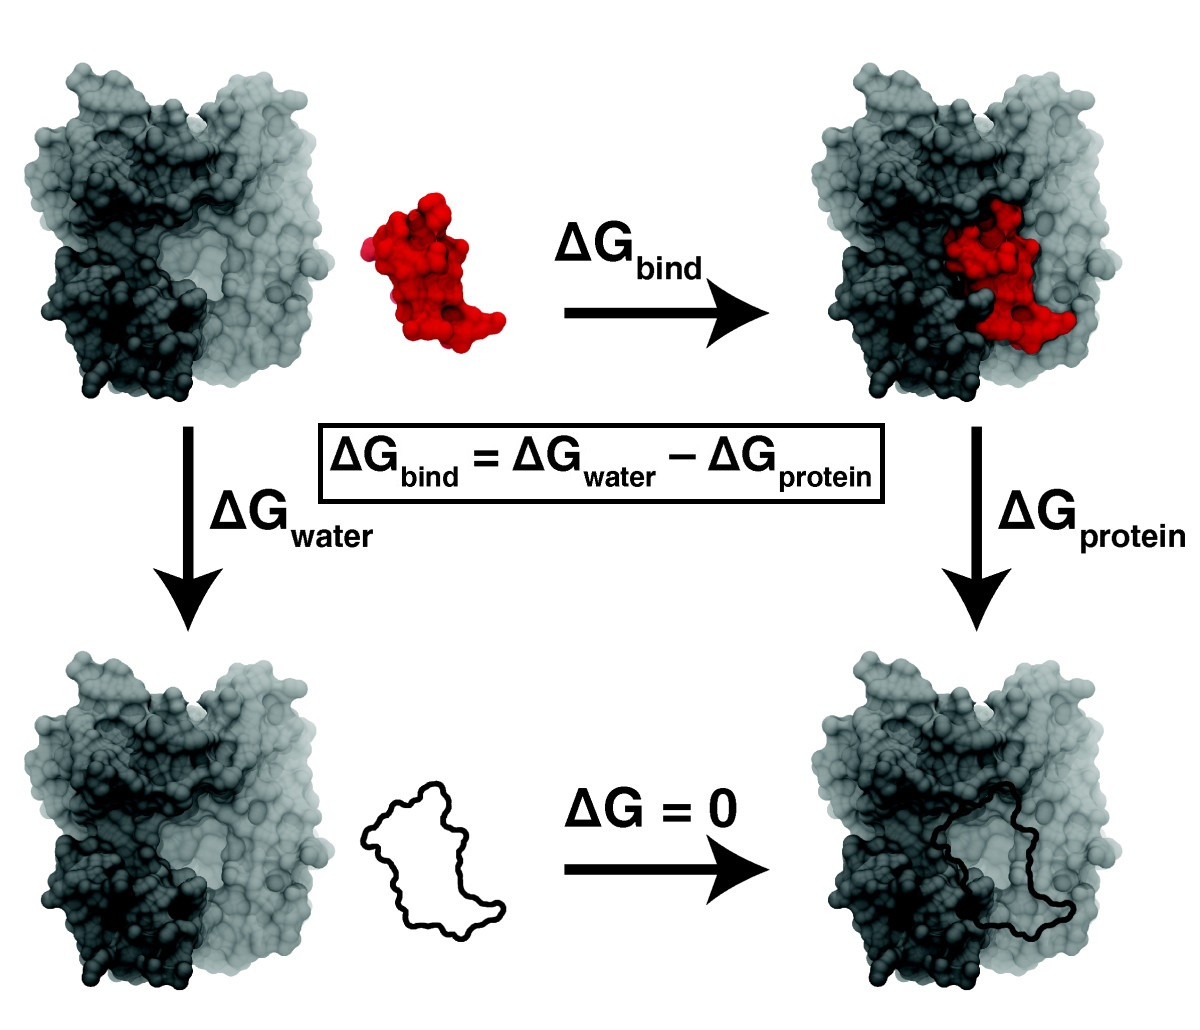
\includegraphics[scale=0.9]{thermcycle-cropped.jpg}
\caption[The thermodynamic cycle]{The thermodynamic cycle, adapted from Durrant and McCammon\cite{durrant2011molecular}}
\label{thermcycle}
\end{figure}

However, free energy is a state function, and as a result, $\Delta G_{bind}$ can be expressed as the sum of an alternate set of free energies along a different path, as illustrated in the thermodynamic cycle in figure \ref{thermcycle}. This alternate pathway involves the computation of two free energies of solvation, $\Delta G_{water}$ and $\Delta G_{protein}$, both of which depend only on small conformational changes accessible to MD, such as side chain rotations, which occur on the \si{\pico\second} to \si{\nano\second} scale\cite{harvey2012high}.

\section{Bridge sampling, the BAR estimator and beyond}
\label{barsubsec}

The problem of directly calculating $\Delta G_{bind}$ has been recast as the problem of indirectly calculating $\Delta G_{bind}$ via the thermodynamic cycle. Given a collection of sampled conformations, what remains is the second phase of free energy calculation: estimation. A wide variety of estimators exist\cite{shirts2007alchemical,pohorille2010good,christ2010basic}, but it has been shown that asymptotically, estimators derived from bridge sampling methods, notably the Bennett acceptance ratio (BAR)\cite{bennett1976efficient}, are unbiased and have the lowest variance of known estimators\cite{shirts2007alchemical,shirts2003equilibrium,shirts2008statistically}. Additionally, in empirical tests, BAR has been shown to outperform competing algorithms, specifically exponential averaging (EXP) and thermodynamic integration (TI)\cite{shirts2005comparison}.

Bridge sampling is a generalized form of BAR from the statistics literature, used for estimating ratios of normalizing constants\cite{meng2002warp,gelman1998simulating,meng1996simulating}. The bridge sampling identity is:
\begin{equation} \label{bridgesamE}
r \equiv \frac{c_1}{c_2} = \frac{E_2[q_1(w)\alpha(w)]}{E_1[q_2(w)\alpha(w)]}
\end{equation}

\noindent where $c_i$ is the normalizing constant, $\alpha(w)$ is an arbitrary function, and $E_i$ denotes the expectation with respect to $p_i$. Given a set of draws from $p_1$ and $p_2$, the ratio estimate is:
\begin{equation} \label{bridgesam}
\hat{r}=\frac{\frac{1}{n_2}\sum_{j=1}^{n_2}q_1(w_{2j})\alpha(w_{2j})}{\frac{1}{n_1}\sum_{j=1}^{n_1}q_2(w_{1j})\alpha(w_{1j})}
\end{equation}

\noindent where $\{w_{i1}, ..., w_{in}\}$ are draws from $p_i$, $i=1,2$.

Equation \eqref{bridgesam} defines the bridge sampling class of estimators for a range of $\alpha$ functions. BAR is defined by the choice of $\alpha$ as: 
\begin{equation}
\alpha ~\propto~ (s_1 q_1+s_2 r q_2)^{-1}
\end{equation}

\noindent where $s_i=n_i/(n_1+n_2)$. This $\alpha$ minimizes the asymptotic variance of $\log(\hat{r})$ as well as the asymptotic relative variance, $E(\hat{r}-r)^2/r^2$, when the draws are independent\cite{meng2002warp}. As $\alpha$ depends on the unknown ratio, iterative methods are used to estimate $r$\cite{meng1996simulating}.

From equation \eqref{bridgesamE}, it is apparent that when the phase space overlap between $p_1$ and $p_2$ is small, the variance of $\hat{r}$ will be large: the expectations are dominated by rare sampling events in the small overlap region. For macromolecules, small phase space overlap is the rule, rather than the exception\cite{wu2005phase1,wu2005phase2}. To remedy this, a series of intermediate distributions can be introduced to increase the overlap between adjacent states\cite{shirts2007alchemical}. These intermediates are termed ``alchemical intermediates," as these distributions define non-physical entities: fictitious molecules whose potential functions are defined as a mixture between those of the two real, physical endpoints. A collection of alchemical intermediates connecting two distributions of interest is called an alchemical path. The most widespread alchemical intermediate generation scheme is $\lambda$-scaling\cite{shirts2007alchemical,christ2010basic}:
\begin{equation} \label{lambdascaling}
U_{\lambda}(\boldsymbol{x}, \lambda)= (1-\lambda) U_1(\boldsymbol{x}) + \lambda U_2(\boldsymbol{x})
\end{equation}

\noindent $\lambda$ varies between 0 and 1, allowing for a range of potential functions from those defining the real systems $U_1$ or $U_2$ for $\lambda$ equals 0 and 1 respectively, to some intermediate, alchemical system when $\lambda$ takes any other value. The unnormalized density is given by:
\begin{equation}
q_\lambda(\boldsymbol{x}, \lambda) = \exp(-\beta U_\lambda(\boldsymbol{x}, \lambda))
\end{equation}

\noindent The introduction of intermediate distributions provides a way to approach ratio estimation with a divide and conquer strategy. Until the phase space overlap between adjacent states is sufficient for reliable ratio estimation, alchemical intermediates can be introduced to further improve overlap and simplify the estimation problem. The result of a single division is illustrated below:
\begin{equation} \label{tbar}
\begin{split}
\Delta G = G_2-G_1 &= (G_2-G_i) + (G_i-G_1) \\
 &= -\beta^{-1}\log(Z_2/Z_i) -\beta^{-1}\log(Z_i/Z_1) \\
 &= -\beta^{-1} \log\left(\frac{Z_2}{Z_i} * \frac{Z_i}{Z_1}\right) \\
 &= -\beta^{-1} \log\left(\frac{Z_2}{Z_1}\right)
\end{split}
\end{equation}

\noindent where $G_i$ and $Z_i$ respectively represent the free energy and partition function of an alchemical intermediate, $i$. For an arbitrary number of intermediates, the telescoping product form in the penultimate line of \eqref{tbar} remains equivalent to the desired ratio in the final line. 

\section{Alchemical intermediate selection}

Careful alchemical intermediate selection has been the focus of several research efforts in the chemical physics literature\cite{pham2011identifying,lu1999optimal,blondel2004ensemble,resat1993studies}, but a widely accepted and used method for intermediate selection is yet to emerge\cite{wu2005phase2}. For the alchemical intermediate generation scheme defined in equation \eqref{lambdascaling}, there are two fundamental choices to be made: how many alchemical intermediates to generate, and which $\lambda$ values they will take. Suggested methods for intermediate selection range from specific Gaussian quadrature rules\cite{AMBER14manual}, to loose guidelines recommending a two step process\cite{shirts2007alchemical}, to dynamic $\lambda$ variation in slow growth methods\cite{pearlman1989new}. For one dimensional path sampling, Gelman and Meng\cite{gelman1998simulating} derive an expression for the optimal prior density.

\begin{figure}
    \centering
    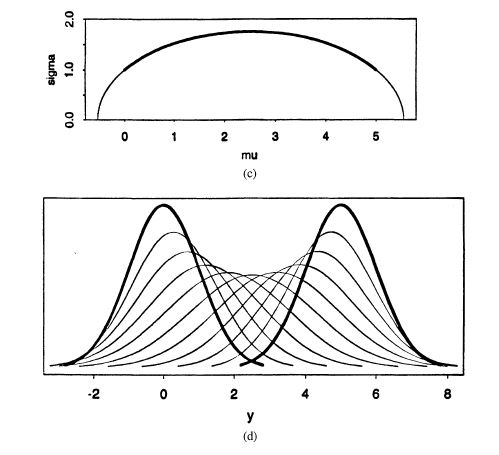
\includegraphics[scale=0.6]{pathsampling.jpg}
    \caption[Gelman and Meng's optimal bridging densities for normal distributions]{Figure from Gelman and Meng (1998). Optimal path from $\mathcal{N}(0,1)$ to $\mathcal{N}(5,1)$ in ($\mu, \sigma$) space. Top panel: Parameter representation. Bottom panel: Density representation for selected intermediates.}
    \label{GMnormnorm}
\end{figure}

In the same study, Gelman and Meng reported an even more striking result, shown in figure \ref{GMnormnorm}.
For a transition between normal distributions with continuous paths, by expanding the distribution space to allow both the mean and variance to vary, as opposed to only the mean, a new minimum variance path was found that outperformed the optimal direct one dimensional solution. For alchemical intermediate selection, multivariate representations of the potential are analogous to this expansion of the distribution space. The intermediate selection problem becomes more difficult, but with a larger potential payoff.
% pathsearch.tex

\chapter{Optimal Path Determination by Exhaustive Search}
\label{chap:dijkstra}

\section{Defining an augmented $\lambda$ space}

In order to ascertain the impact of Gelman and Meng's result on alchemical intermediate selection for free energy calculations, we must first define in which way to expand the alchemical state space defined by equation \eqref{lambdascaling}. 
Numerous options exist, including separation of energy terms (Jiang \& Roux\cite{jiang2010free}) and the addition of a biasing potential (Darve et al.\cite{darve2008adaptive}), but the most natural choice is to expand the alchemical space using a temperature parameter (Sugita et al.\cite{sugita2000multidimensional}).

Using temperature as a second dimension in the alchemical state space confers numerous and predictable benefits, both practically and technically. 
Varying temperature in the alchemical space confers similar benefits to replica exchange molecular dynamics (REMD), an expanded ensemble sampling method designed to overcome energetic barriers\cite{sugita2000multidimensional}, and because temperature is a standard tunable parameter in molecular simulation packages, sampling states in this expanded space comes at no additional cost, implementation-wise.

As defined, the potential energy is not dependent on temperature, but the unnormalized density is affected:

\begin{equation} 
q_{\lambda,\beta}(\boldsymbol{x}, \lambda, \beta) = \exp(-\beta U_{\lambda}(\boldsymbol{x},\lambda))
\label{eqn: alchemical distr}
\end{equation}

\noindent Consequently, the partition function $Z_{\lambda, \beta}$ will also depend on the temperature.

While temperature is a convenient thermodynamic parameter for our purposes, letting temperature vary introduces some issues as well. Free energy differences between two states can be expressed as the log ratio of partition functions as in \eqref{freeeneqn} and \eqref{tbar} only when the two states are at the same temperature. This imposes the constraint that the end points of our alchemical path, the real physical systems of interest, must be at the same temperature.
%, but this was always the case for biologically motivated calculations.
%requirement is not problematic: it was already implicit in other methods.
What must be verified is that intermediate alchemical states can pass through regions of varying temperature while still recovering the telescoping product in \eqref{tbar}. Revisiting \eqref{tbar} when the temperature of the intermediate is given by $\beta_i$:
\begin{equation} \label{tempfail}
\Delta G=(G_2-G_i) + (G_i-G_1) = [-\beta^{-1} \log(Z_1) + \beta_i^{-1} \log(Z_i)] + [-\beta_i^{-1}\log(Z_i) +\beta^{-1}\log(Z_0)]
\end{equation}

\noindent It clear that we cannot estimate this free energy difference using BAR type methods if $\beta_i \neq \beta$.
To resolve this problem, we can define $G_i^\ast$ as scaled free energies for intermediate states:
\begin{equation} \label{Gscale}
G_i^\ast = \beta_i/\beta *G_i = \beta_i/\beta * (-\beta_i^{-1} \log(Z_i)) = -\beta^{-1} \log(Z_i)
\end{equation}

\noindent Replacing $G_i$ with $G_i^\ast$ in \eqref{tempfail} will recover the telescoping product, as in \eqref{tbar}.

It is therefore important to note that in this expanded alchemical space, we are not computing sums of ``correct" free energies along the alchemical path, but ``improper" free energies. 
Only the sum of free energies along a complete path is physically meaningful.
Nevertheless, this expanded space has been shown to be well suited to relative free energy calculations using BAR, since these improper free energies allow for the estimation of a telescoping product of normalizing constants, which are unaffected by the scaling in \eqref{Gscale}.

\section{Revisiting Gelman and Meng in discrete state spaces}

To demonstrate the existence of better paths in our augmented $(\lambda, T)$ space, we sought out to recreate Gelman and Meng's result in our discrete state space. 
We can define a normal distribution in our scheme by creating a harmonic well, with $U(x)=(x-a)^2$, where $a=\mu$ , and the temperature and variance are related as $T ~\propto~ \sigma^2$. We set our endpoint states to be $p_0\sim\mathcal{N}(0,1)$ and $p_1\sim\mathcal{N}(5,1)$.

By using Dijkstra's algorithm\cite{dijkstra1959note}, we can exactly determine the minimum cost path connecting our $\lambda_0$ and $\lambda_1$ states. In accordance with the qualitative interpretation of \eqref{bridgesamE}, total variation distance was used as a measure of the overlap between two distributions. The optimal path maximizes the overlap between adjacent distributions, and minimizes the sum of total variation distances along the path. 

\begin{figure}
\centering
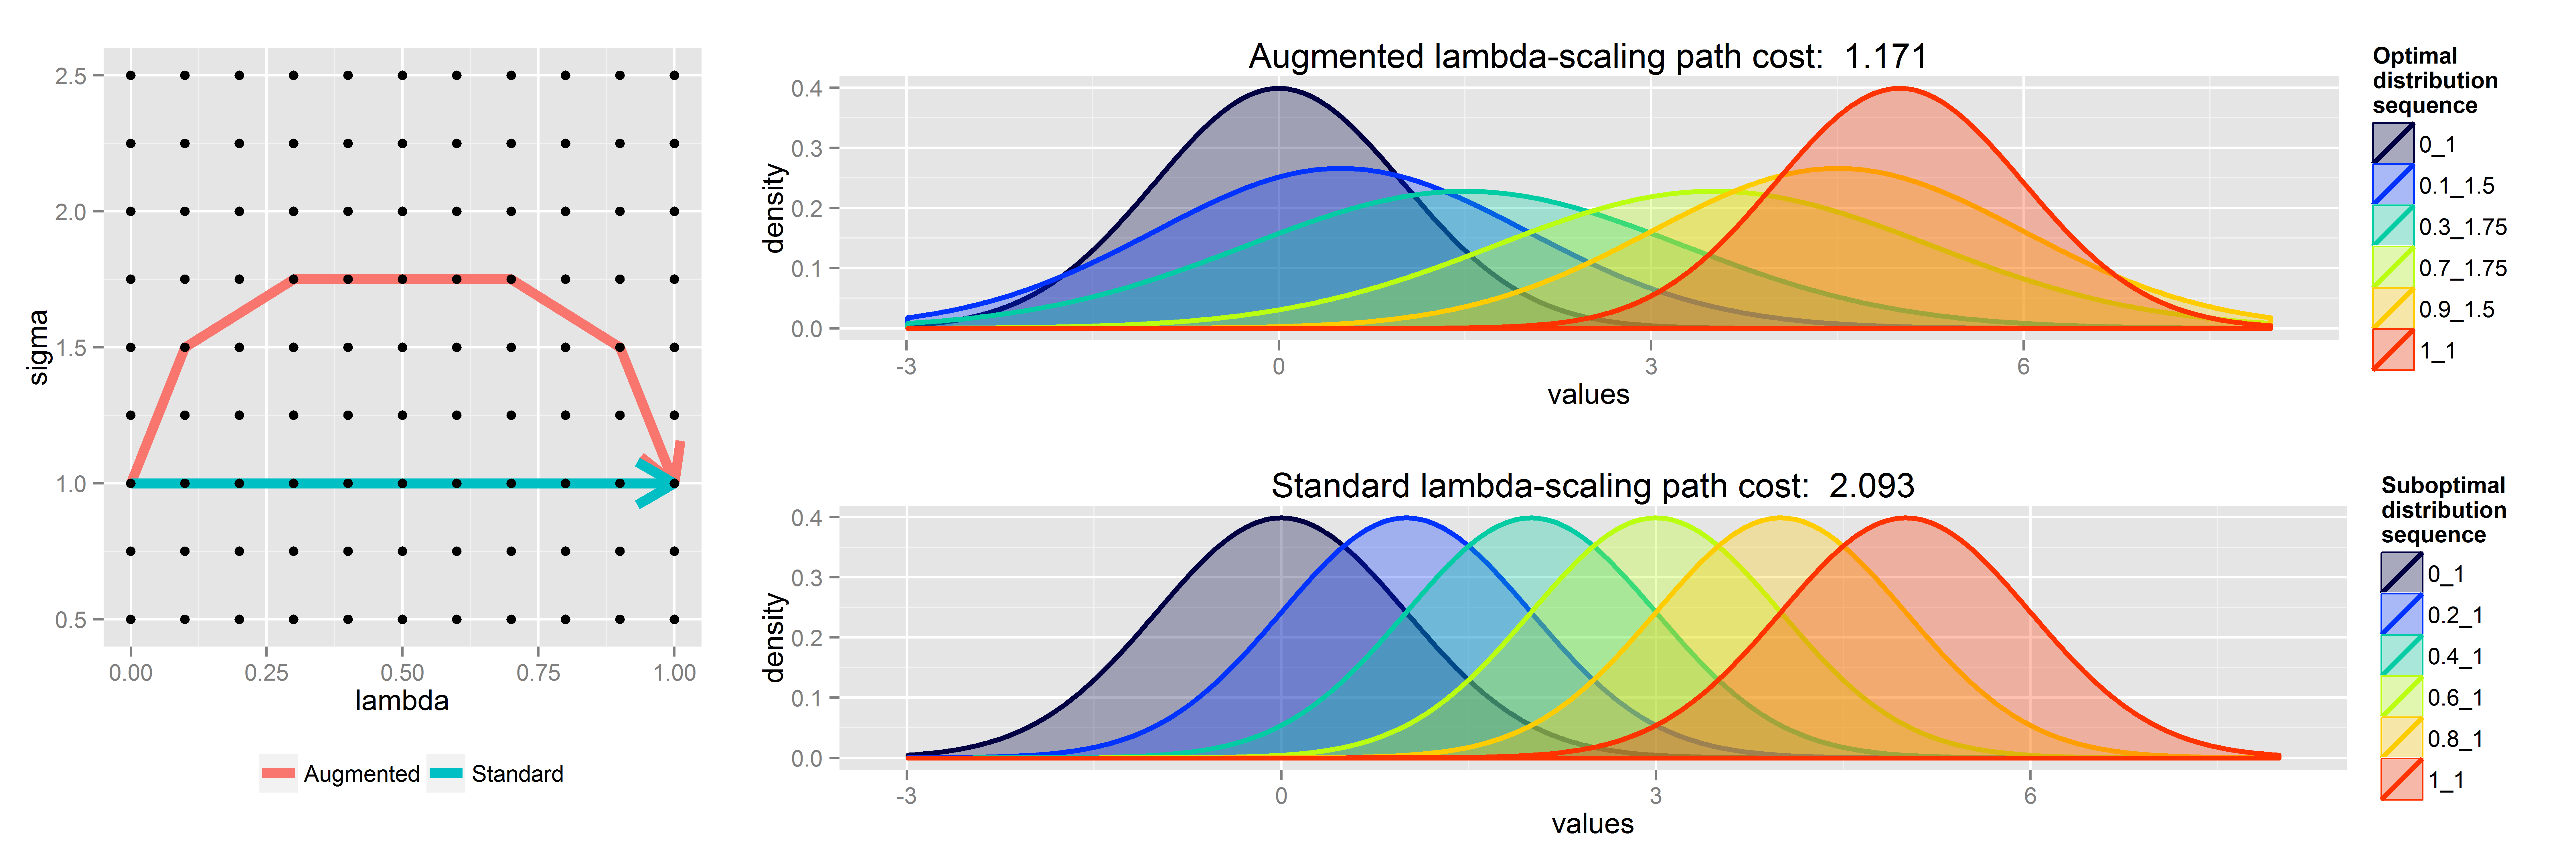
\includegraphics[scale=0.4]{unimod-3pan-searchv2.png}
\caption[Dijkstra search on total variation distance for offset harmonic wells]{Dijkstra search on total variation distance for offset harmonic wells. Left panel: Parameter representation of paths. Optimal path for temperature augmented $\lambda$-space in red. Optimal path for standard, one dimensional, $\lambda$ space in blue. Right panel: Density representation of paths. Top panel: distributions along optimal path flatten with increased temperature. Path cost of 1.171. Bottom: distributions along standard path simply mean shift. Path cost of 2.093.}
\label{uniuni}
\end{figure}

The result of the search are shown in figure \ref{uniuni}. We show that in discrete spaces, the Gelman and Meng result holds. An ellipsoid path which raises the temperature for intermediate distributions is the overall optimal path. These results confirm that not only is the standard path suboptimal, but that it is direly so. The path cost of the best standard solution is 2.093, which is nearly a two-fold increase from the globally optimal solution of 1.171.

To confirm the general utility of the augmented $\lambda$ space, we repeated the above search for a different target distribution, representing an increase in complexity. We set $U_1(x) ~\propto~ (ax^4-bx^2)$, where $a$ and $b$ are arbitrary scalars, to create a bimodal distribution. 
The result of this search, shown in figure \ref{unibi}, is consistent with that from figure \ref{uniuni}. The general shape of the optimal path appears to be somewhat conserved: high temperature regions are leveraged to increase distributional overlap.

\begin{figure}
\centering
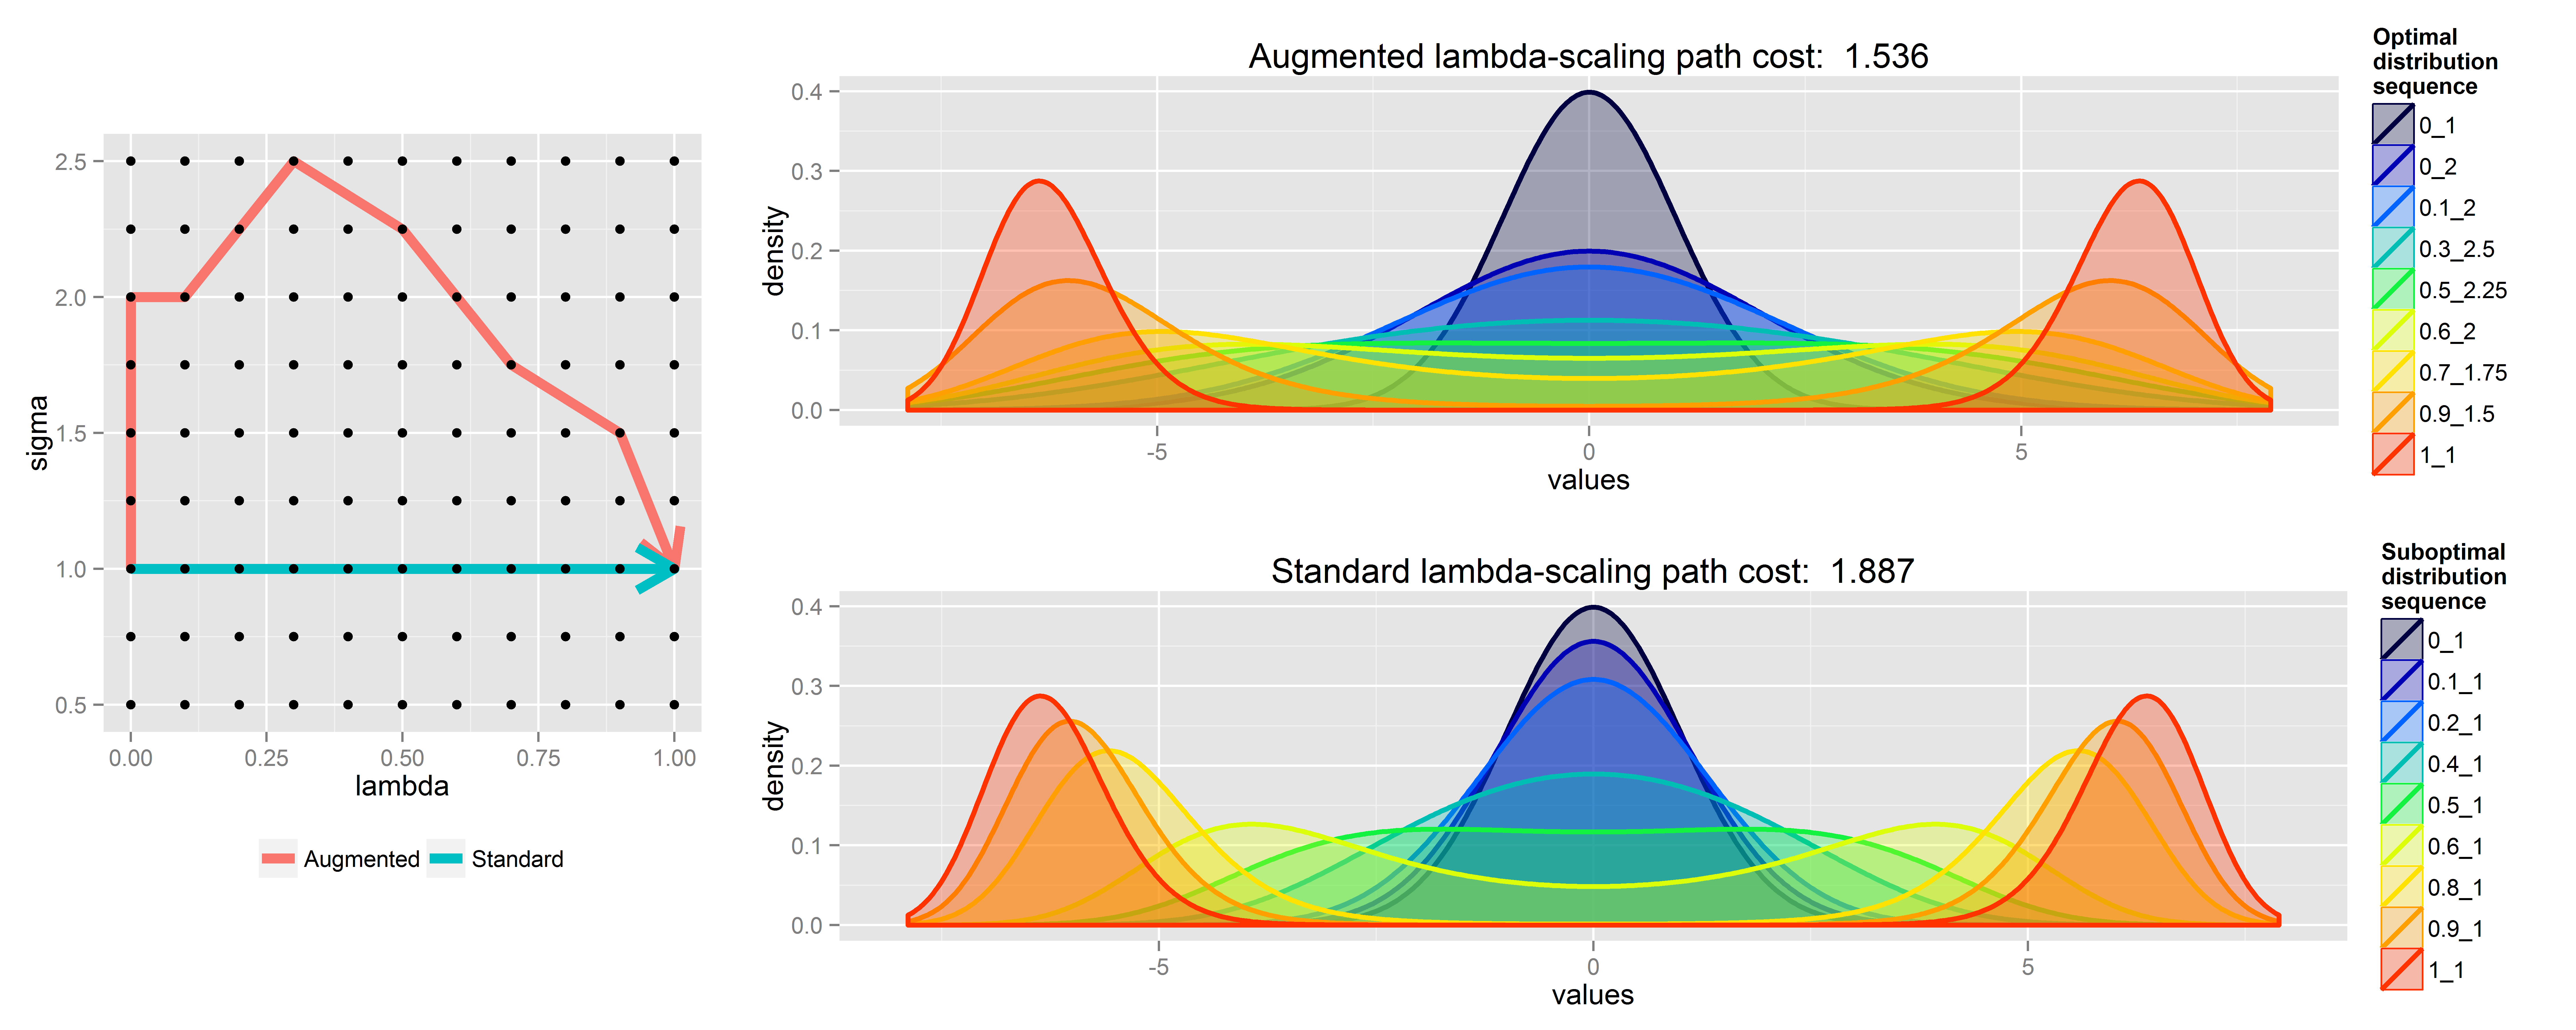
\includegraphics[scale=0.4]{unib1-3pan-searchv1.png}
\caption[Dijkstra search on total variance distance for the normal to bimodal transformation]{Dijkstra search on total variance distance for the normal to bimodal transformation. Panels mirror those from figure \ref{uniuni}. Optimal path cost: 1.536. Standard path cost: 1.887.}
\label{unibi}
\end{figure}

\section{Moving towards free energy calculations}

\subsection{A proper distance metric - varBAR}

In the previous section, we used total variation distance as edge weights in the graph search. 
While informative, this does not accurately reflect the type of information available for macromolecular systems. 
As the goal of a free energy calculation is to minimize the variance of the free energy estimate, a more appropriate distance metric is exactly that: the variance of the BAR estimate between adjacent states (hereafter the varBAR distance).
For the BAR estimator, an expression for the asymptotic variance of the free energy difference (or equivalently, the relative variance of the ratio estimate) was derived by Shirts and his colleagues\cite{shirts2008statistically, shirts2003equilibrium}:

\begin{equation} \label{eq:varbar}
    \text{var}(\Delta \hat{f}) = \frac{\text{var}(\hat{r})}{r^2} = \frac{1}{N}\left [ \left \langle \frac{1}{2+2\cosh(\Delta \hat{f} - \Delta u(x) -M)} \right \rangle ^{-1} - \left ( \frac{N}{N_2} + \frac{N}{N_1} \right ) \right ]
\end{equation}

\noindent where $M=\ln N_1/N_2$. Empirical tests show that this expression returns accurate variance estimates even for limited sample sizes.% (data not shown).

\begin{figure}
    \centering
    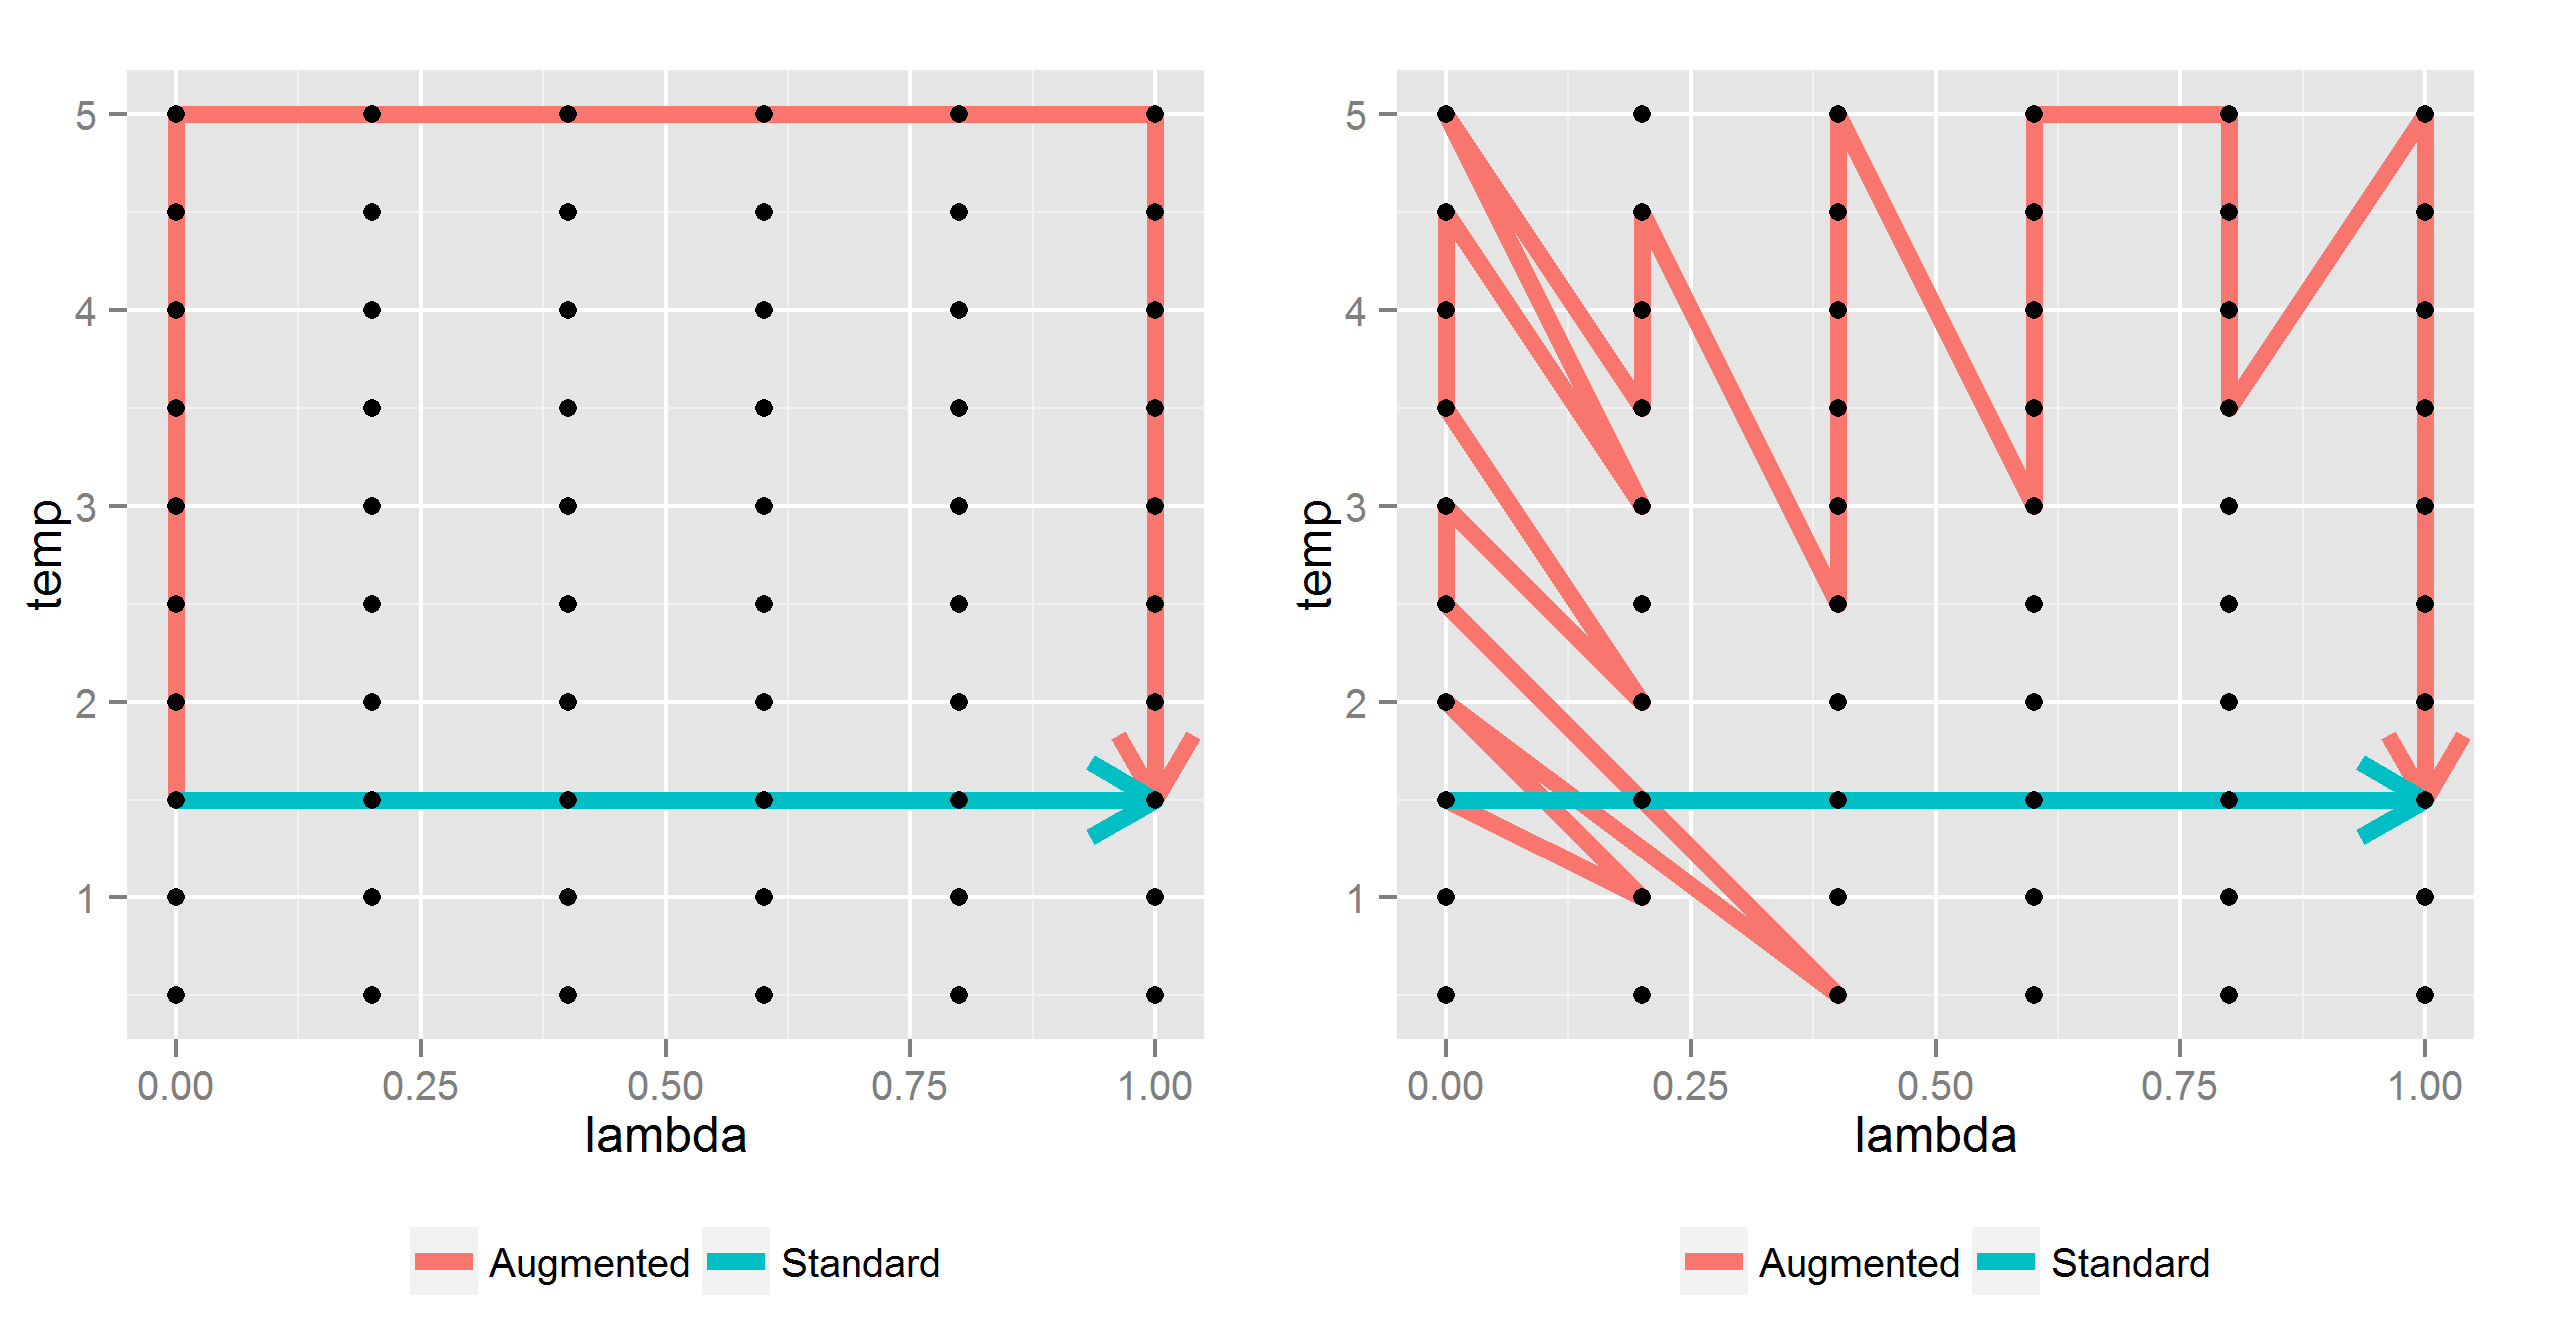
\includegraphics[scale=0.2]{varBAR-paramviews.png}
    \caption[Dijkstra search on varBAR distance]{Parameter representation of paths for Dijkstra search on varBAR distance for offset harmonic wells (left) and normal to bimodal transformation (right). See text for path costs.}
    \label{varbar-paramviews}
\end{figure}

Figure \ref{varbar-paramviews} summarizes the search results using this new objective function for the previously examined test cases. 
For the normal to normal case, the optimal path cost is 5.13E-4, and the standard path cost is 1.58E-3. For the normal to bimodal case, the optimal path cost is 3.93E-4, and the standard path cost is 1.81E-3.
While the variance is substantially reduced in both cases (approximately 70\% and 80\% reduction in variance respectively), we note that both optimal paths contain many intermediate states.
In a molecular simulation context, these paths would incur a much higher sampling cost, due to the number of intermediate states requiring simulation.
Indeed, if we add intermediates to the standard path to match the number of intermediates in the optimal paths, the benefit of the augmented space becomes unclear. 
The standard path costs for the normal to normal and normal to bimodal cases become 3.88E-4 and 2.18E-4, respectively.

\subsection{Cost adjusted paths}

In order to make sound comparisons, we must put a constraint on the total amount of computation, or equivalently, fix the total number of drawn samples across all paths being compared. 
In an equilibrium sampling context, depending on the total number of edges in a path, the number of available draws on each constituent state will vary, and consequently the cost of an edge will vary, due to variance scaling with N, as seen in \eqref{eq:varbar}. 
This dependence on global properties of the path on individual edge costs breaks the dynamic programming Dijktra's algorithm is built on.

To properly optimize these equal cost paths, we use a modified version of Dijkstra's algorithm, which constrains paths to a fixed length, then carry out a search for a range of possible path lengths. % http://stackoverflow.com/questions/1690347/shortest-path-with-a-fixed-number-of-edges
By prespecifying the number of edges in the solution path, we can determine the number of samples per state, and scale all edge costs appropriately for a recursive dynamic programming search.

\begin{figure}
    \centering
    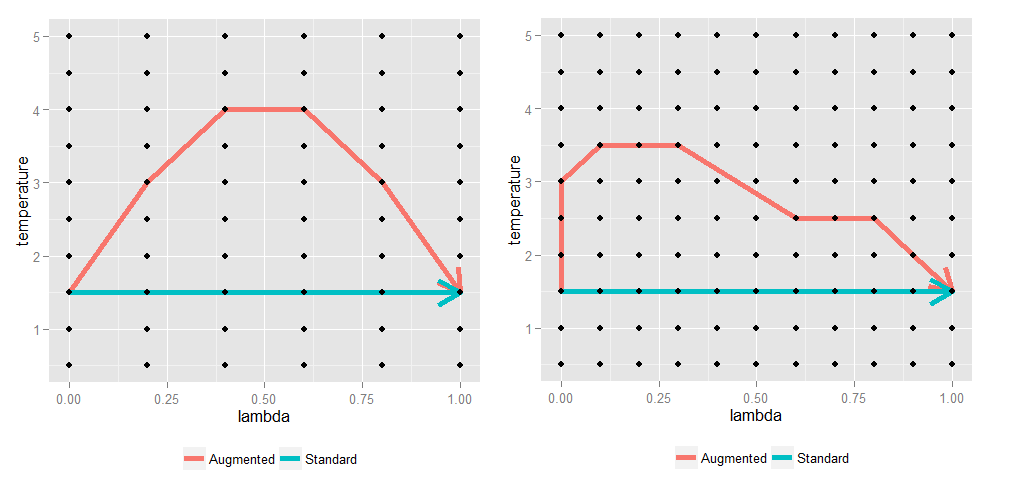
\includegraphics[scale=0.55]{kshortest.png}
    \caption[Cost-adjusted Dijkstra search]{Parameter representation of paths for cost-adjusted Dijkstra search on varBAR distance for offset harmonic wells (left) and normal to bimodal transformation (right). See text for path costs.}
    \label{fig:kshortest}
\end{figure}

Figure \ref{fig:kshortest} shows the optimal paths when varBAR costs account for the total number of edges in the path. 
For the offset harmonic well, the standard path cost is 5.07E-4, and the augmented path cost is 3.18E-4. 
For the unimodal to bimodal case, the standard path cost is 7.03E-5, and the augmented path cost is 5.93E-5.
We note that these corrected paths regain some of the smoothness that we had observed in figures \ref{uniuni} and \ref{unibi}.


\section{Scalability of Dijkstra's algorithm to molecular systems}

The results from this chapter serve as a proof of concept and establish the validity and theoretical utility of the temperature augmented state space for free energy calculations, however Dijkstra's algorithm is not suitable for path optimization going forward.
Dijkstra's algorithm requires knowledge of every edge weight in the graph.
Consequently, in order to apply Dijkstra's algorithm, a sufficient number of samples must be drawn from each alchemical state.
For molecular systems, this type of exhaustive search is cost prohibitive, and a path searching methodology which balances exploration and exploitation to discover and refine paths online is necessary. 
We will revisit our options for path selection in chapter \ref{chap:ql}.


% smc.tex

\chapter{Sequential Monte Carlo for Free Energy Estimation}
\label{chap:smc}

Path optimization in free energy calculations comes in several forms. 
In chapter \ref{chap:dijkstra}, we explored the possibility of optimizing the intermediates that make up the path, in order to minimize the variance and decrease the required number of samples needed to reach a desired precision.
In this chapter, we will approach optimization from a complementary angle. 
Given a fixed alchemical path, can we reduce the computational cost per sample, and can we construct an efficient estimator with the minimum variance properties of BAR?

There is considerable overlap between chemical physics studies on free energy calculations and research in statistics for estimating ratios of normalizing constants. 
Indeed, as we pointed out with the relationship between BAR and bridge sampling, methods from the statistics literature have previously been adapted for use in biophysical problems.

Nonequilibrium methods, such as Jarzynski's method\cite{jarzynski1997nonequilibrium1}, have gone largely underappreciated in the chemical physics literature despite their statistical equivalent, sequential Monte Carlo\cite{cappe2007overview, del2006sequential} (SMC), enjoying widespread use.
A key benefit of SMC methods that we would like to leverage in molecular simulation is the enormous reduction in computational cost for sampling.
For equilibrium sampling, assuming a system relaxation time of $\tau$ and $k$ alchemical states in the path, to obtain $n$ draws would require $\mathcal{O}(\tau k n)$ computation.
On the other hand, for nonequilibrium sampling, we only require $\mathcal{O}(\tau n)$ time to generate initial configurations from one equilibrium simulation, then through a series of cheap nonequilibrium moves, we generate weighted particle trajectories in time $\mathcal{O}((k-1)\tau^\prime n)$, for a total cost of $\mathcal{O}((\tau + (k-1)\tau^\prime)n)$, where $\tau >> \tau^\prime$. 

\section{Combining bridge sampling and SMC}

The primary downside of Jarzynski's method and its statistical analogue, annealed important sampling\cite{neal2001annealed} (AIS), is that while the sample collection step is rapid, the ratio estimation step is inefficient. 
This is because these are one-sided estimators, which only use draws from one target state, of which the most well known is Zwanzig's exponential averaging\cite{zwanzig1954high}:

\begin{equation}
    \Delta G_{0 \rightarrow 1} = -\beta^{-1} \log E_0[\exp(-\beta(U_1(x)-U_0(x))]
\end{equation}

To remedy this statistical inefficiency, we develop a modified version of BAR, that we call sequential BAR (seqBAR, or sBAR), which uses the BAR estimation step with rapidly generated SMC particles.
This fusion of SMC and bridge sampling methods is enabled by a resampling step\cite{murray2012gpu}, which transforms weighted SMC particles into a collection of draws approximating the equilibrium distribution for every intermediate state.
These resampled particles can then be used directly in BAR estimation as in equation \eqref{bridgesam}. 

\begin{figure}
    \centering
    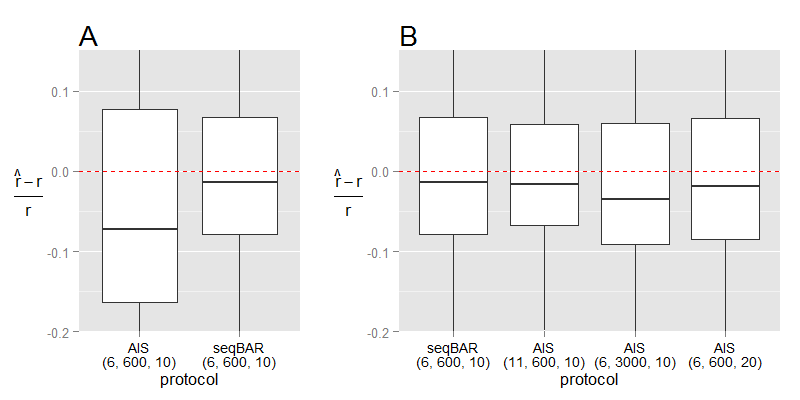
\includegraphics[scale=0.7]{seqBARvAIS-uni-bi-v02.png}
    \caption[Comparison of seqBAR and AIS performance for the normal to bimodal transformation]{Comparison of seqBAR and AIS performance for the normal to bimodal transformation. Performance is judged by the empirical accuracy and precision of the relative error of the ratio estimate for 500 independent realizations. Protocols are defined by an estimation method (AIS or seqBAR), followed by a trio of parameters, indicating respectively, the number of distributions in the path, the number of sample trajectories, and the number of Metropolis mixing steps per transition. Left panel: Comparison of AIS and seqBAR performance for equal computation time. Right panel: Required computation for AIS to match seqBAR performance.}
    \label{fig:sBARvAIS}
\end{figure}

Figure \ref{fig:sBARvAIS} demonstrates the gains in statistical efficiency when using seqBAR over AIS. 
For equal computation, seqBAR is, on average, closer to the true ratio value, and has more consistent ratio estimates, from replicate to replicate. 
To match the performance of seqBAR, AIS requires either a doubling of the number of distributions in the path, a five-fold increase in the number of samples, or a doubling in the cost of each nonequilibrium transition, here a Metropolis\cite{metropolis1953equation} mixing step.

\section{SMC in the augmented $(\lambda, T)$ space}
\label{sec:smcpath}

SMC methods are also sensitive to path choice. 
For the normal to normal example, five paths in the $(\lambda, T)$ space were compared using AIS. 
Ratio estimates, squared errors and estimated variances are shown in figure \ref{fig:AIS-pathcompare}.
We note that there appears to be a tradeoff with using the higher temperatures. 
As temperature increases up to a maximum value of 3 (a path height of 2), AIS performance improves. 
Once temperature increases beyond that point (path heights 3 and 4), the increased temperature introduces too much noise, and the variance of the ratio estimate increases, even beyond that of an AIS run using the standard, fixed temperature path.

\begin{figure}
    \centering
    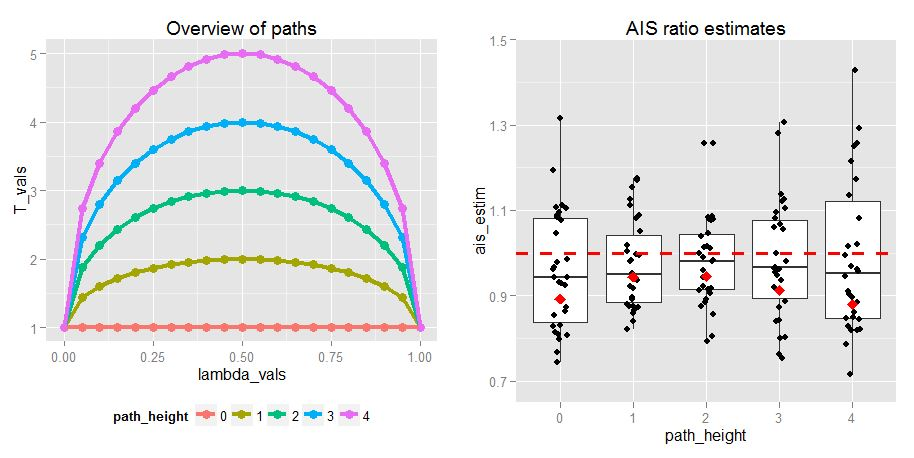
\includegraphics[scale=0.6]{ais-pathcompare.jpg}
    \caption[Comparison of AIS paths for offset harmonic wells]{Comparison of AIS paths for offset harmonic wells. Left: parameter space representation of paths. Right: ratio estimates indexed by path. The dotted red line denotes the true ratio. Red diamonds represent average values for each path height.}
    \label{fig:AIS-pathcompare}
\end{figure}

\section{pCrooks: a pairwise decomposable CFT}
\label{sec:pcrooks}

Regardless of path, there are conditions under which AIS and seqBAR can struggle, namely when the target distributions are sufficiently different such that nonequilibrium moves are unable to create particles approximating the final distribution. 
One such example is the transition from a normal distribution to a Cauchy distribution (t-distribution with one degree of freedom), due to their differing tail decay rates.
In the same way that BAR improves on exponential averaging by creating bridge functions and utilizing samples from both target distributions, the Crooks fluctuation theorem\cite{crooks2000path} (CFT) improves on Jarzynski's method. 
CFT is a a hybrid SMC-bridge sampling method, which operates on nonequilibrium work distributions generated in both sampling directions.
This bidirectional propagation results in increased robustness to varying target distributions for ratio estimation, as seen in figure \ref{fig:pcrooks}.
Note that both AIS and seqBAR are highly variable, and frequently under estimate the ratio, whereas CFT (crooks) is extremely accurate.

\begin{figure}
    \centering
    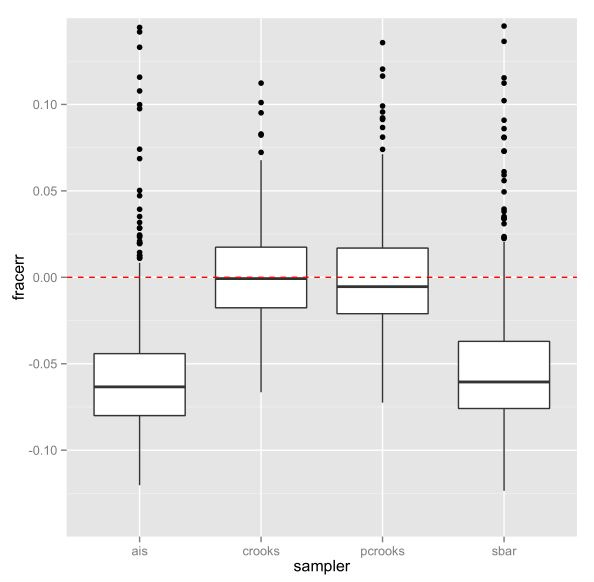
\includegraphics[scale=0.6]{pcrooks.jpg}
    \caption[Comparison of various SMC methods for the normal to Cauchy transformation]{Comparison of AIS, CFT, pCrooks and seqBAR ratio estimation performance for the normal to Cauchy distribution transformation.}
    \label{fig:pcrooks}
\end{figure}

In the context of path selection however, CFT has notable shortcomings. 
For path selection between enumerated (and frequently non-overlapping) paths, CFT is acceptable, but when trying to optimize paths in a full grid search, when there may be significant barriers to work around, and we have no guesses as to what form an acceptable path may take, the dependence on CFT on full path work distributions hinders our ability to locally optimize transitions and build reasonable paths.
To this end, we developed pairwise Crooks (pCrooks), a pairwise decomposable version of CFT. 
Instead of using full path work distributions to estimate the full telescoping ratio in one step, we calculate each pairwise ratio using BAR with weighted work distributions, where the weights are derived from the accumulated SMC transitions.
In figure \ref{fig:pcrooks}, we show that pCrooks corrects the shortcomings of seqBAR, and approaches the effectiveness of CFT.
By breaking down the ratio estimation step, we can obtain information on the variance of each transition in the path, allowing us to locally optimize the path, and refine existing paths, by trying other transitions to replace high variance links.


% ql.tex

\chapter{Path Selection via Reinforcement Learning}
\label{chap:ql}

Exhaustive search by Dijkstra's algorithm in chapter \ref{chap:dijkstra}, and empirical benchmarking in section \ref{sec:smcpath} have demonstrated the theoretical utility of an augmented state space. 
In practice however, the principal challenge is to efficiently navigate the augmented state space to find improved paths without offsetting the gains in efficiency afforded by those paths.
We draw on machine learning techniques from the reinforcement learning literature to address this task.

\section{SMC and the multi-armed bandit}

The multi-armed bandit problem\cite{tokic2011value, scott2010modern, vermorel2005multi} is an optimization problem originating from probability theory. 
Selecting between an enumerated set of paths for free energy estimation can be cast as a sample allocation problem, where the conflicting goals of drawing samples for estimation along the putative best path and drawing samples for estimating the quality of other potentially better paths are in opposition. 
In figure \ref{fig:aisbandit}, we examine our ability to optimize paths with SMC by comparing three bandit strategies. 

\begin{figure}
    \centering
    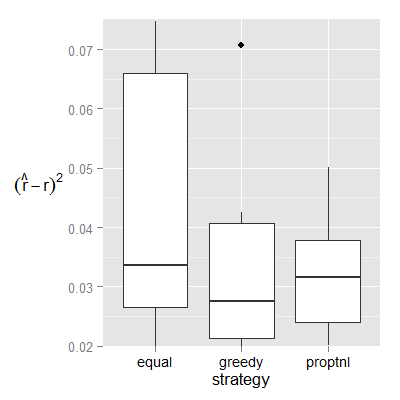
\includegraphics[scale=0.7]{ais-bandit.png}
    \caption[Comparison of three AIS bandit strategies]{Comparison of squared error for three AIS bandit strategies for offset harmonic wells. See text for details on strategies.}
    \label{fig:aisbandit}
\end{figure}

The ``equal'' strategy is effectively the null strategy, where each path is sampled equally, regardless of their estimated variances.
The ``greedy'' strategy follows up an initial exploration period of equal sampling with a period where only the minimum estimated variance path is sampled.
The ``proptnl'' strategy follows up an initial exploration period of equal sampling with a period where each path is sampled in quantities inversely proportional to their variances.
We observe that the greedy strategy is, on average, the strategy that minimizes the squared error of the ratio estimate, however it is also interesting to note that the proportional strategy is the most consistent one.

A weakness of this form of path selection, as we alluded to in section \ref{sec:pcrooks}, is that it only operates on fully predefined paths.
As we saw in figure \ref{fig:kshortest}, the shape of the optimal path can vary, and as the dimensionality of the underlying distributions increases, it is possible that the optimal paths will become more irregular in order to navigate around energetic barriers. 
In these situations, where we have no intuition to guide path definition, selection between enumerated paths may not be sufficient for the efficiency gains we seek, and a full grid optimization is required, where a path is built edge by edge.

\section{Full grid optimization with Q-learning}

Q-learning\cite{watkins1992q} is a reinforcement learning technique for finite state Markov decision processes, typically used to derive an optimal action selection policy for total reward maximization.
Q-learning progresses through successive learning episodes, where a $Q$ function describing the expected values of the long term rewards for each state-action pair is inferred via value iteration updates. Search agent actions, and the putative best path are both guided by the current best estimate of the $Q$ function, which is updated as follows after each search episode:

\begin{equation}
    Q_{t+1}(s,a) = Q_t(s,a) + \alpha (R(s,a) + \gamma \max_{a^\prime}Q_t(s^{\prime}, a^{\prime}) - Q_t(s,a))
\end{equation}

\noindent where $\alpha \in [0,1]$ is the learning rate, $\gamma \in [0,1]$ is a discount factor to penalize delayed rewards, $R(s,a)$ is a function that returns some reward for the action $a$ out of state $s$, and the maximum is the maximum $Q$ value for all actions out of the resulting state for the observed action.

In our application, as our goal is to minimize the variance of the path, the reward function $R(s,a)$, represents estimated variances for a given transition between states. 
These variance estimates are given by equation \eqref{eq:varbar} for a low cost pCrooks run.
Ratio estimates for a given transition from separate learning episodes can be combined as a mean weighted by their inverse variances.

To make Q-learning compatible with a minimization task, we make two important adjustments in order to minimize the accumulated reward.
First, we take the minimum $Q$ value over the resulting states, instead of the maximum.
Second, $\gamma$ now takes values of 1 or higher.
This second adjustment is required to avoid situations where Q-learning will create infinite loops in the solution path to delay a required large cost action. 
In a minimization context, when $\gamma$ is bounded by 0 and 1, longer paths are favored, as distal costs become discounted. 
As we've previously seen, longer paths come at a larger computational cost, so we constrain $\gamma$ to be 1 or larger, to favor shorter paths. 
$\gamma$ can be tuned to reflect the relative cost of equilibrium sampling and nonequilibrium SMC transition moves, where values near one represent low cost SMC moves.

\subsection{Fixed duration Q-learning} % (fold)
\label{sub:fixed_duration_q_learning}

In this section, Q-learning is run for a preselected number of learning episodes, representing a fixed ceiling on the amount of available computation time.
$\alpha$ is set to 0.8, and $\gamma$ is set to 1.
The search space is the augmented $(\lambda, T)$ space for the offset harmonic wells. 

\begin{figure}
    \centering
    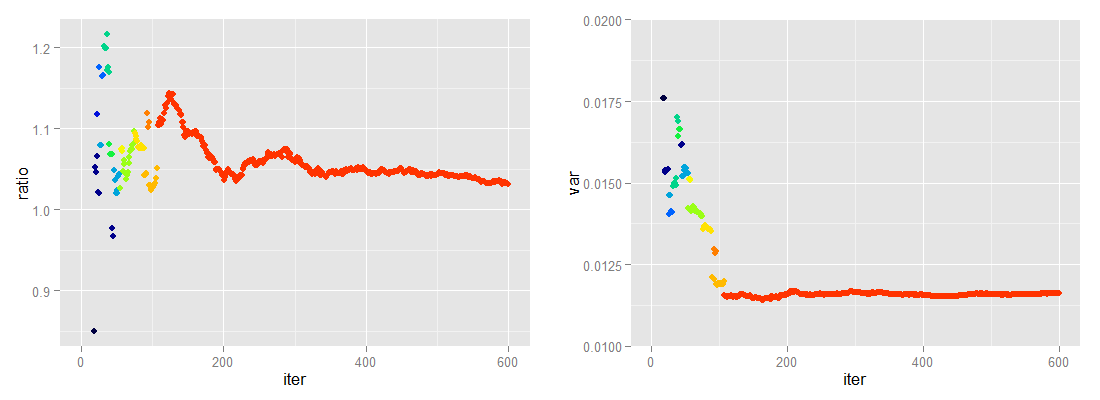
\includegraphics[scale=0.5]{ql-monitor-chain1.png}
    \caption[Ratio and variance estimates monitored for fixed duration Q-learning]{Ratio and variance estimates monitored for fixed duration Q-learning. Target distributions are offset harmonic wells, $\alpha=0.8, \gamma=1$. Changes in point color represent changes in the current best path.}
    \label{fig:ql-summary}
\end{figure}

Figure \ref{fig:ql-summary} shows the evolution of the ratio estimates, variance estimates, and current best path as a function of the number of learning episodes that have elapsed.
For the first 100 steps of the algorithm, the best guess optimal path varies rapidly, as denoted by the changing point colors.
As the algorithm progresses, path variance estimates become more precise, and the low cost paths are learned by the $Q$ function, as illustrated by the decreasing variance in the second panel, and the fixation of the red path as the optimal path.
The ratio estimation converges near the true value of 1. 

\begin{figure}
    \centering
    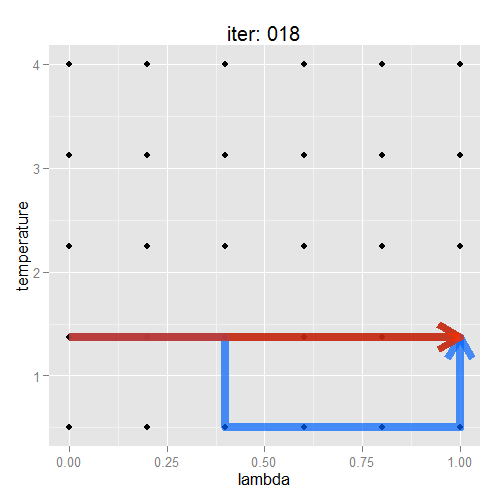
\includegraphics[scale=0.35]{iter-018.png}
    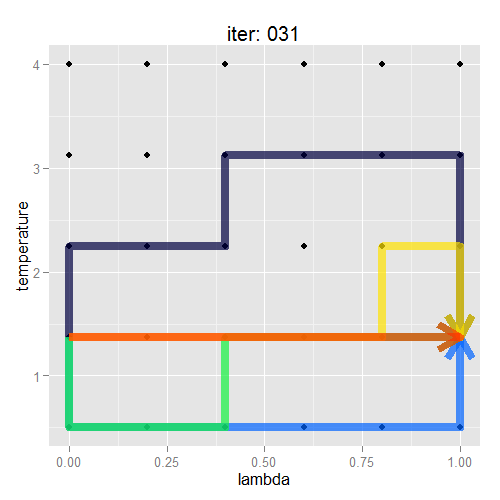
\includegraphics[scale=0.35]{iter-031.png}
    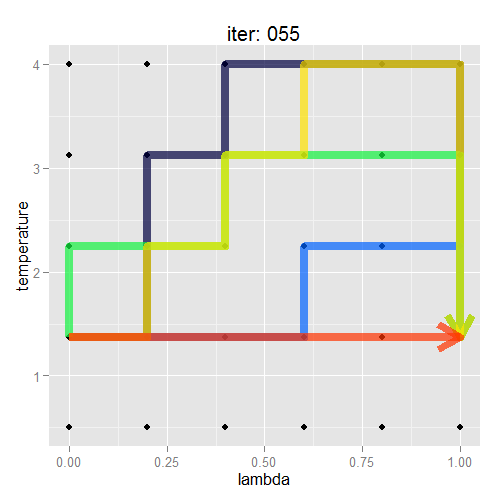
\includegraphics[scale=0.35]{iter-055.png} \\
    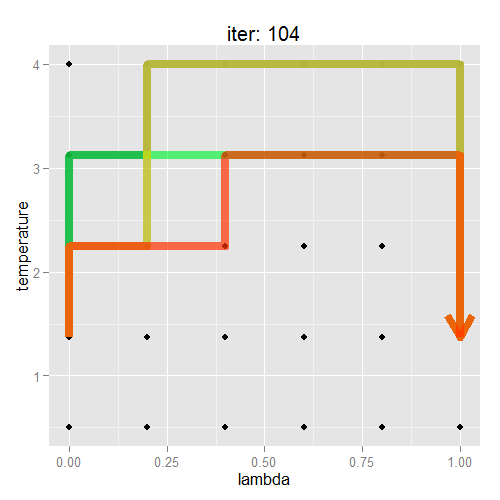
\includegraphics[scale=0.35]{iter-104.png}
    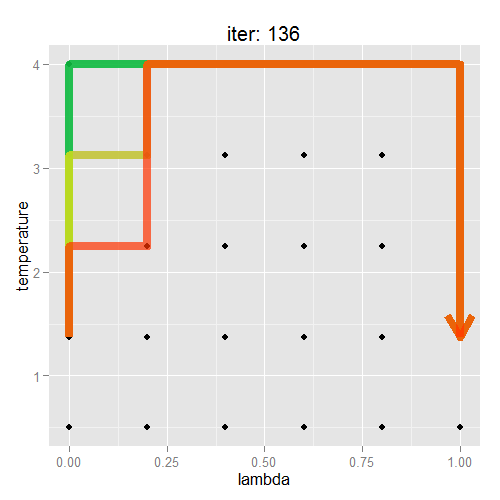
\includegraphics[scale=0.35]{iter-136.png}
    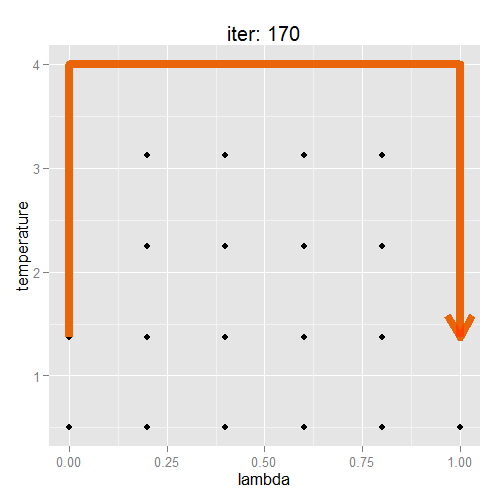
\includegraphics[scale=0.35]{iter-170.png}
    \caption[Time evolution of five Q-learning chains]{Time evolution of five Q-learning chains for offset harmonic wells. $\alpha=0.8, \gamma=1$. Each panel shows the current best path as determined by independent runs of Q-learning at different time points. Clockwise from top left: 18, 31, 55, 170, 136 and 104 iterations elapsed.}
    \label{fig:ql-slices}
\end{figure}


Figure \ref{fig:ql-slices} depicts the evolution of the best guess path for five replicates of the Q-learning algorithm on this test case.
Each color represents one chain's best guess path varying across iterations.
At the 18th iteration, only some replicates have determined a complete best path. These paths are direct, and not necessarily low variance. In fact, the path in blue is a higher variance path than the standard, fixed temperature path.
At the 31st iteration, all chains have found solution paths, but their forms vary wildly. 
Some, like the dark blue path, are promising in their use of the higher temperature regions.
By the 55th iteration, almost all paths are improved relative to the standard, fixed temperature path. 
The 104th and 136th iterations show that the chains are beginning to converge on similar solution paths. In the 136th iteration, some have even found the true optimal path we had determined by exhaustive search in figure \ref{varbar-paramviews}.
By the 170th iteration, all chains have converged on the true optimal path.
% subsection fixed_duration_q_learning (end)

\subsection{Q-learning convergence} % (fold)
\label{sub:q_learning_convergence}

The goal of a free energy calculation is to obtain an estimate of maximum precision in a set amount of time, or an estimate of set precision in a minimum amount of time.
A downside of Q-learning, and of path selection algorithms in general, is that it divides sampling efforts among many paths during the search phase, and not all of the generated SMC particles will participate in the ratio estimation if the distribution they approximate does not lie on the putative best path.
A benefit of standard $\lambda$ scaling is that all particles traverse only one path, ensuring full sample utilization, and a full reduction in variance by a factor of N.

In this section, we account for this variance reduction factor, and determine if Q-learning can converge on an improved path fast enough to offset particle waste in the early stages of the algorithm.
For both an augmented and standard state space, we run three independent Q-learning chains. 
For the standard state space, this entails simply running a free energy estimation along the fixed temperature path, as there are no alternative paths to consider.
After each iteration, we construct a composite free energy estimate based on the three chain estimates.
Within a predefined tolerance level, we assess if the individual chains agree with this composite estimate, based on a chain interval derived from the chain estimate and variance.
Chain concordance with the composite estimate provides a heuristic check for free energy estimate convergence.

\begin{figure}
    \centering
    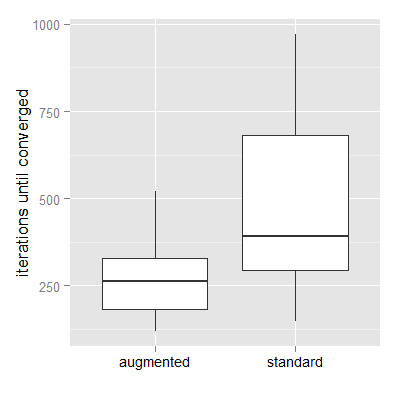
\includegraphics[scale=0.7]{ql_conv.png}
    \caption[Rates of Q-learning convergence]{Rates of Q-learning convergence for offset harmonic wells. $\alpha=0.8, \gamma=1$. For 30 replicates each, convergence rates for Q-learning in the temperature-augmented and standard state spaces are compared. The free energy estimates converge signficantly faster with path searching enabled via Q-learning, relative to when path searching is disabled, with the standard state space.}
    \label{fig:ql-convergence}
\end{figure}

The results of testing this convergence heuristic are shown in figure \ref{fig:ql-convergence}.
Despite the computational overhead Q-learning in the augmented state space incurs, it still converges significantly faster and at a more consistent rate than free energy estimation along the standard path.
On average, when path searching is permitted, convergence is achieved 1.8 times faster than when free energy estimation is confined to a fixed temperature path.
This result shows that path selection by Q-learning, in conjunction with free energy estimation with pCrooks is a valid approach for practical path optimization.

% subsection q_learning_convergence (end)

% discussion.tex

\chapter{Discussion}

Multivariate representations of state spaces have enjoyed great success for sampling, both in a molecular dynamics context with replica-exchange molecular dynamics\cite{sugita2000multidimensional}, and in a statistical context with hybrid Monte Carlo\cite{duane1987hybrid}.
In this work, we have motivated an analogous extension to free energy calculations.
Inspired by the work of Gelman and Meng\cite{gelman1998simulating}, we showed that the addition of a temperature parameter to the $\lambda$ scaling alchemical generation scheme allows for the creation of new, reduced variance alchemical paths.
Furthermore, we found that Q-learning\cite{watkins1992q}, a reinforcement learning technique, could be successfully adapted for use as an algorithm for simultaneous path optimization and free energy estimation.

In parallel work, we expanded on the work of Jarzynski\cite{jarzynski1997nonequilibrium1} and Crooks\cite{crooks2000path} to develop a new nonequilibrium sampler and free energy calculation method, which we call pCrooks. 
pCrooks is fundamentally a bridge sampling method, like CFT, but unlike CFT, pCrooks provides information on the variance for each pair of adjacent states in an alchemical path, making it a method that synergizes well with path optimization algorithms. 

This document serves as a proof of concept for these methods.
For simple models, where exhaustive or analytical methods are feasible, we determined reference values against which to test our methods, and showed that we were able to efficiently recover these solutions with our methodology.
The combined algorithm with Q-learning for path optimization and pCrooks as a subroutine for sampling and free energy estimation represents the culmination of this work.
In a head to head comparison, our path optimizing Q-learning algorithm was able to converge on a free energy estimate at significantly lower computational cost than the fixed path alternative.

This result is notable because it demonstrates the practical applicability of path optimization in free energy calculations, even in situations where little is known about the energy landscape of the alchemical state space.
For large molecular systems, where the standard path may run into wide regions of poor overlap, characterized by significant energy barriers, this path optimization may provide a method for avoiding these difficult and problematic transitions.

Moving forward, to fully realize the potential of this method, further testing must be done to determine if the path searching will remain efficient for more complex distributions.
Reasonable next test cases range from those where a known barrier exists, such as in a ferromagnetic Ising model\cite{mora2012transition}, to well studied examples from the free energy calculation literature, such as the free energy of solvation of methane\cite{paliwal2011benchmark}, or relative binding free energies to T4 lysozyme\cite{boyce2009predicting}.

To deal with the task of sampling high dimensional energy functions, the SMC sampling protocol may require additional improvements. 
A bidirectional sampling method, like pCrooks, can be combined with a resampling step as is used in seqBAR to alleviate issues related to minimal density overlap.
Further expansions to the alchemical state space should be considered with caution. 
As the dimensionality of the state space grows, the overhead associated with Q-learning's path searching will increase rapidly.

In summary, we hope that this work will represent the beginning of a paradigm shift in alchemical intermediate selection away from unprincipled, rule of thumb methods, and towards heuristic methods which take into account the properties of the underlying state space determined by low cost pilot simulations.


% % introduction.tex

\chapter{Introduction}

The free energy difference between two states is a highly sought after quantity, as it determines their macroscopic behavior. The states can be constructed with flexibility, such that we can obtain information about various phenomena including, but not limited to, protein binding and protein folding. Given current methods and computational resources, free energy calculations for biologically relevant macromolecules remain impractical\cite{shirts2007alchemical, pohorille2010good}.

This impracticality arises due to the heavy cost of sampling conformations for large molecular systems. An ideal sampler for free energy calculations will address the two main challenges current samplers face. First, it must sample the entire configuration space efficiently. The sampler must be able to move across regions of low density to sample a multitude of potential wells. Second, it must collect draws from not only the two systems of interest, but also a series of intermediate distributions which provide a sequence of maximum overlap, connecting the two systems of interest.

The objective of this research is to develop an efficient sampler that will negotiate these challenges, making reliable free energy calculations for macromolecules possible. To meet this goal, three avenues are explored. 
The first aim of this research is to explore alternative, multivariate parameterizations of the potential function that are suitable for polypeptide systems. I demonstrate this idea by adding a temperature parameter to the classic $\lambda$-scaling intermediate distribution generation scheme. This increased dimensionality makes the sampler more flexible, at the cost of an increase in the difficulty of determining good sequences of intermediate distributions. For several simple models of increasing complexity, an exhaustive graph search over the space of intermediate distributions is used to determine the best set of bridging densities (hereafter, the optimal path), revealing the benefits of this more flexible scheme. 

The second aim of this research is to develop a low cost sampling method compatible with the path searching paradigm introduced in the first aim.
Crooks\cite{crooks2000path} and Jarzynski\cite{jarzynski1997nonequilibrium1} have previously explored the application of Sequential Monte Carlo (SMC) samplers\cite{del2006sequential, cappe2007overview} to free energy estimation, and generated renewed interest in cost efficient nonequilibrium sampling.
We present a new sampling and estimation algorithm, pCrooks, a pairwise extension of the Crooks Fluctation Theorem (CFT), which maintains the computational benefits of SMC samplers while providing detailed information on each transition in the alchemical path, allowing for interfacing with path optimization algorithms.

In order for the expanded state space from the first aim to be practical, the cost of finding an improved path must be less than the gains afforded by its use. 
Computational effort must be allocated between the competing tasks of drawing samples for free energy estimation and drawing samples for path space exploration.
In the third aim, we apply reinforcement learning techniques, such as Q-learning\cite{watkins1992q}, to efficiently optimize the path without incurring a large sampling burden and computational cost for the exploration phase.
}
% \include{{./Chapter2/guide-notes}} % A regular chapter, starts with '\chapter{Title}'
% \include{{./Chapter3/chRegularLook}}
% \include{{./Chapter4/chLorem}}
% \include{{./Chapter5/chLorem2}}
%==============================================================================

%-----------------------------------------------------------------------------%
% APPENDICES -- OPTIONAL. These are just chapters enumerated by Appendix A,
%                Appendix B, Appendix C...
%-----------------------------------------------------------------------------%
\appendix
% detmeth.tex

% detailed methods for the appendix of the duke thesis

\chapter{Detailed Methods}

This appendix contains detailed method descriptions and parameter values required to reproduce the work shown in this thesis. \\
Code is available at \url{https://github.com/rmuraglia/Schmidler}.
% \begin{verbatim} https://github.com/rmuraglia/Schmidler \end{verbatim}.

\section{Exhaustive search} % (fold)
\label{sec:exhaustive_search}

\subsection{Dijkstra's algorithm} % (fold)
\label{sub:dijkstra_s_algorithm}

Dijkstra's algorithm is a dynamic programming algorithm for finding minimum cost paths through graphs

% subsection dijkstra_s_algorithm (end)

\subsection{Fixed path length search} % (fold)
\label{sub:fixed_path_length_search}

% subsection fixed_path_length_search (end)

% section exhaustive_search (end)
% \include{{./Appendix1/chLorem3}} % Start with '\chapter{Title}'
%You can always add more appendices here if you want

%-----------------------------------------------------------------------------%
% BIBLIOGRAPHY -- uncomment \nocite{*} to include items in 'mybib.bib' file
% that aren't cited in the text.  Change the style to match your
% discipline's standards.  Of course, if your bibliography file isn't called
% 'mybib.bib' you might want to change that here too :)
%-----------------------------------------------------------------------------%
% \nocite{*} %- if you use this it will put EVERYTHING in your .bib file into the references even if you don't cite it in the text
\bibliographystyle{unsrt} %Formats bibliography
% \bibliographystyle{./Bibliography/jasa}
\cleardoublepage
\normalbaselines %Fixes spacing of bibliography
\addcontentsline{toc}{chapter}{Bibliography} %adds Bibliography to your table of contents
\bibliography{./Bibliography/prelimrefs}
% \nocite{durrant2011molecular}

% \bibliography{./Bibliography/References} %your bibliography file - change the path if needed
%-----------------------------------------------------------------------------%

%-----------------------------------------------------------------------------%
% BIOGRAPHY -- Start file with '\biography'.  Mandatory for Ph.D.
%-----------------------------------------------------------------------------%
% \include{{./Biography/biography}}

%-----------------------------------------------------------------------------
% You're done :)
\end{document}
